\section{Capítulo 6 -- Grafos}

A árvore do Capítulo 5 representa hierarquias: cada nó tem um único pai. Muitas relações, porém, não têm hierarquia nenhuma. Uma cidade se liga a várias outras por estradas, uma pessoa é amiga de várias outras, uma página da web aponta para muitas páginas, e todas podem formar ciclos. A estrutura que representa qualquer rede de ligações é o \textbf{grafo}. Neste capítulo você vai aprender a guardar um grafo na memória, a percorrê-lo e a resolver dois problemas clássicos: encontrar o caminho mais curto e ligar todos os pontos com o menor custo.

\subsection{6.1 Vértices e arestas}

Um grafo é formado por um conjunto de \textbf{vértices} (os pontos) e um conjunto de \textbf{arestas} (as ligações entre pares de vértices). Uma árvore é um caso particular de grafo: um grafo conectado e sem ciclos.

As arestas podem ter ou não um sentido:

\begin{center}
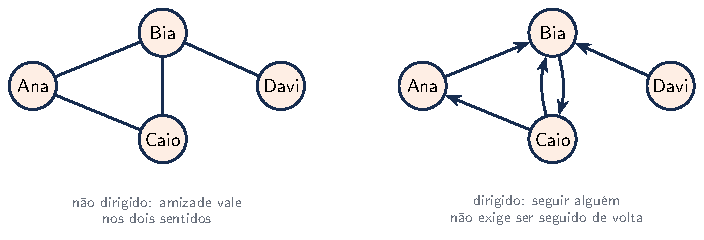
\includegraphics[width=0.9\linewidth,keepaspectratio]{imagens/capitulo-06_tipos.pdf}
\end{center}

\begin{itemize}
  \item Em um grafo \textbf{não dirigido}, a aresta liga os dois vértices nos dois sentidos, como uma amizade ou uma estrada de mão dupla.
  \item Em um grafo \textbf{dirigido} (ou \textbf{dígrafo}), cada aresta tem origem e destino e é desenhada como uma seta, como ``seguir'' alguém em uma rede social ou um pré-requisito entre disciplinas.
\end{itemize}

Quando cada aresta tem um número associado, como uma distância, um tempo ou um custo, o grafo é \textbf{ponderado}, e esse número é o \textbf{peso} da aresta. O grafo abaixo será usado como exemplo em todo o capítulo: seis cidades e as estradas entre elas, com as distâncias em quilômetros.

\begin{center}
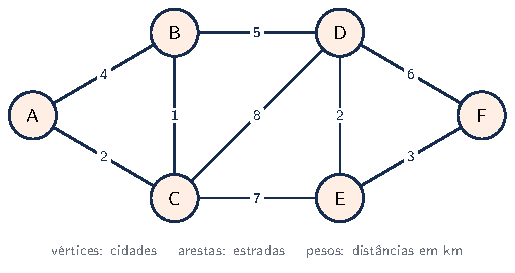
\includegraphics[width=0.8\linewidth,keepaspectratio]{imagens/capitulo-06_grafo.pdf}
\end{center}

\begin{center}
\begin{tabular}{@{}p{0.24\linewidth}p{0.68\linewidth}@{}}
\toprule
\rowcolor{headergray}
\tblheader{Termo} & \tblheader{Significado} \\
\midrule
adjacentes (vizinhos) & dois vértices ligados por uma aresta; no exemplo, B e D \\
\rowcolor{rowgray} grau & número de arestas de um vértice; o grau de C é 4 \\
caminho & sequência de vértices em que cada um é vizinho do seguinte, como A, C, E, F \\
\rowcolor{rowgray} ciclo & caminho que começa e termina no mesmo vértice, como A, B, C, A \\
conexo & grafo em que existe caminho entre quaisquer dois vértices \\
\rowcolor{rowgray} componente conexo & cada ``pedaço'' de um grafo que não é conexo \\
\bottomrule
\end{tabular}
\end{center}

Nos algoritmos, é costume chamar o número de vértices de $V$ e o número de arestas de $E$ (do inglês \textit{edges}). O exemplo tem $V = 6$ e $E = 9$.

\subsection{6.2 Representando um grafo}

Existem duas formas principais de guardar um grafo na memória. Para numerá-los, os vértices recebem índices: A é 0, B é 1, e assim por diante.

\subsubsection{Matriz de adjacência}

A \textbf{matriz de adjacência} é uma tabela $V \times V$ em que a posição \texttt{[i][j]} diz se existe aresta de \texttt{i} para \texttt{j} (ou guarda o peso dela). No grafo de amizades da primeira figura:

\begin{codigo}
\begin{Verbatim}[breaklines=true, breaksymbolleft={}, fontsize=\footnotesize]
int main() {
    const int N = 4;
    const string nomes[N] = {"Ana", "Bia", "Caio", "Davi"};
    bool amigos[N][N] = {};                  // começa tudo false

    amigos[0][1] = amigos[1][0] = true;      // Ana e Bia
    amigos[0][2] = amigos[2][0] = true;      // Ana e Caio
    amigos[1][2] = amigos[2][1] = true;      // Bia e Caio
    amigos[1][3] = amigos[3][1] = true;      // Bia e Davi

    cout << boolalpha << amigos[0][3] << endl;   // false: consulta em O(1)

    for (int v = 0; v < N; v++) {
        int grau = 0;
        for (int u = 0; u < N; u++) {        // percorre a linha inteira: O(V)
            if (amigos[v][u]) grau++;
        }
        cout << nomes[v] << ": " << grau << endl;   // Ana: 2, Bia: 3, Caio: 2, Davi: 1
    }
}
\end{Verbatim}
\end{codigo}

Em um grafo não dirigido, a matriz é \textbf{simétrica}: cada aresta é marcada duas vezes. A vantagem é saber em $O(1)$ se dois vértices são vizinhos. A desvantagem é a memória: são sempre $V^2$ posições, mesmo que haja poucas arestas. Uma rede social com um milhão de pessoas precisaria de um trilhão de posições, quase todas \texttt{false}.

\subsubsection{Lista de adjacência}

A \textbf{lista de adjacência} guarda, para cada vértice, apenas a lista dos seus vizinhos. Em C++, a forma mais simples é um \texttt{vector} de \texttt{vector}s: a posição \texttt{v} contém os vizinhos de \texttt{v}, cada um com o peso da aresta.

\begin{codigo}
\begin{Verbatim}[breaklines=true, breaksymbolleft={}, fontsize=\footnotesize]
// trecho
struct Aresta {
    int destino;
    int peso;
};

class Grafo {
private:
    vector<vector<Aresta>> adjacentes;   // uma lista de vizinhos por vértice

public:
    explicit Grafo(int n) : adjacentes(n) {}

    int vertices() const { return static_cast<int>(adjacentes.size()); }

    void ligar(int a, int b, int peso = 1) {   // aresta não dirigida
        adjacentes[a].push_back({b, peso});
        adjacentes[b].push_back({a, peso});
    }

    const vector<Aresta> &vizinhos(int v) const { return adjacentes[v]; }
};
\end{Verbatim}
\end{codigo}

Repare que não há \texttt{new} nem \texttt{delete}: o \texttt{vector} cuida da própria memória e a libera sozinho quando o grafo deixa de existir. Para um grafo dirigido, basta \texttt{ligar} acrescentar só a primeira das duas linhas.

\begin{center}
\begin{tabular}{@{}p{0.36\linewidth}p{0.26\linewidth}p{0.26\linewidth}@{}}
\toprule
\rowcolor{headergray}
\tblheader{Operação} & \tblheader{Matriz} & \tblheader{Lista} \\
\midrule
memória & $O(V^2)$ & $O(V + E)$ \\
\rowcolor{rowgray} existe aresta entre u e v? & $O(1)$ & $O(\text{grau de u})$ \\
percorrer os vizinhos de v & $O(V)$ & $O(\text{grau de v})$ \\
\rowcolor{rowgray} percorrer o grafo inteiro & $O(V^2)$ & $O(V + E)$ \\
\bottomrule
\end{tabular}
\end{center}

A maioria dos grafos reais é \textbf{esparsa}: cada vértice tem poucos vizinhos em comparação com o total. Por isso a lista de adjacência é a escolha padrão, e é a que usaremos no resto do capítulo. A matriz compensa em grafos pequenos ou \textbf{densos}, com quase todas as arestas possíveis.

\subsection{6.3 Busca em largura}

Percorrer um grafo é mais delicado do que percorrer uma árvore, por dois motivos: não existe uma raiz natural, e os ciclos fazem um vértice ser alcançável por vários caminhos. Para não visitar o mesmo vértice duas vezes, nem entrar em um ciclo infinito, os percursos \textbf{marcam} cada vértice já descoberto.

A \textbf{busca em largura} (BFS, do inglês \textit{breadth-first search}) é a generalização do percurso em largura da árvore. Ela parte de um vértice de origem, descobre todos os seus vizinhos, depois os vizinhos dos vizinhos, e assim por diante, em camadas. Assim como na árvore, quem organiza as camadas é uma \textbf{fila}.

\begin{center}
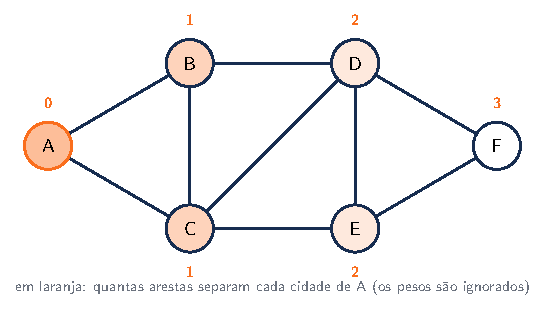
\includegraphics[width=0.8\linewidth,keepaspectratio]{imagens/capitulo-06_largura.pdf}
\end{center}

Como cada camada fica uma aresta mais longe da origem, a BFS calcula, de brinde, o \textbf{menor número de arestas} entre a origem e cada vértice. Em um mapa sem distâncias, ou em uma rede social (``quantos amigos de amigos separam duas pessoas?''), esse é exatamente o caminho mais curto.

\begin{codigo}
\begin{Verbatim}[breaklines=true, breaksymbolleft={}, fontsize=\footnotesize]
// trecho
vector<int> largura(const Grafo &g, int origem, vector<int> &pai) {
    vector<int> distancia(g.vertices(), -1);   // -1: ainda não descoberto
    pai.assign(g.vertices(), -1);
    queue<int> fila;
    distancia[origem] = 0;
    fila.push(origem);
    while (!fila.empty()) {
        int v = fila.front();
        fila.pop();
        for (const Aresta &a : g.vizinhos(v)) {
            if (distancia[a.destino] == -1) {   // primeira vez que aparece
                distancia[a.destino] = distancia[v] + 1;
                pai[a.destino] = v;             // foi descoberto a partir de v
                fila.push(a.destino);
            }
        }
    }
    return distancia;
}
\end{Verbatim}
\end{codigo}

O vetor \texttt{distancia} faz o papel da marcação: $-1$ significa ``ainda não descoberto''. O vetor \texttt{pai} guarda de qual vértice cada um foi descoberto; seguindo os pais a partir de qualquer vértice, você refaz o caminho até a origem. As arestas \texttt{pai}--filho formam uma árvore, chamada \textbf{árvore de busca}.

Cada vértice entra na fila uma única vez, e a lista de vizinhos de cada um é percorrida uma única vez. O custo total é $O(V + E)$.

\subsection{6.4 Busca em profundidade}

A \textbf{busca em profundidade} (DFS, do inglês \textit{depth-first search}) faz o contrário: em vez de avançar em camadas, ela segue um caminho até não haver mais para onde ir e só então volta para tentar outra direção, como alguém explorando um labirinto com a mão sempre na parede. Ela é naturalmente recursiva, e a pilha que guarda o caminho de volta é a própria pilha de execução do Capítulo 4.

\begin{codigo}
\begin{Verbatim}[breaklines=true, breaksymbolleft={}, fontsize=\footnotesize]
// trecho
void profundidade(const Grafo &g, int v, vector<bool> &visitado, vector<int> &pai) {
    visitado[v] = true;
    for (const Aresta &a : g.vizinhos(v)) {
        if (!visitado[a.destino]) {
            pai[a.destino] = v;
            profundidade(g, a.destino, visitado, pai);   // mergulha antes de olhar o próximo vizinho
        }
    }
}
\end{Verbatim}
\end{codigo}

Partindo de A no grafo das cidades, as duas buscas descobrem os mesmos vértices, mas por caminhos bem diferentes. As arestas das árvores de busca mostram isso:

\begin{center}
\begin{tabular}{@{}p{0.28\linewidth}p{0.3\linewidth}p{0.34\linewidth}@{}}
\toprule
\rowcolor{headergray}
\tblheader{Busca} & \tblheader{Árvore de busca} & \tblheader{Formato} \\
\midrule
largura (BFS) & A-B, A-C, B-D, C-E, D-F & larga e baixa: altura 3 \\
\rowcolor{rowgray} profundidade (DFS) & A-B, B-C, C-D, D-E, E-F & um único caminho: altura 5 \\
\bottomrule
\end{tabular}
\end{center}

A DFS também custa $O(V + E)$ e serve de base para muitos algoritmos. Um dos mais simples é \textbf{contar os componentes conexos}: chame a DFS a partir de cada vértice ainda não visitado; cada chamada feita pelo laço principal descobre um componente inteiro.

\begin{codigo}
\begin{Verbatim}[breaklines=true, breaksymbolleft={}, fontsize=\footnotesize]
// trecho
int contarComponentes(const Grafo &g) {
    vector<bool> visitado(g.vertices(), false);
    vector<int> pai(g.vertices(), -1);
    int componentes = 0;
    for (int v = 0; v < g.vertices(); v++) {
        if (!visitado[v]) {                    // começa um grupo novo
            componentes++;
            profundidade(g, v, visitado, pai);
        }
    }
    return componentes;
}
\end{Verbatim}
\end{codigo}

O programa completo monta o grafo das cidades, executa as duas buscas e conta os componentes de uma rede com três grupos separados:

\begin{codigo}
\begin{Verbatim}[breaklines=true, breaksymbolleft={}, fontsize=\footnotesize]
#include <vector>
#include <queue>

struct Aresta {
    int destino;
    int peso;
};

class Grafo {
private:
    vector<vector<Aresta>> adjacentes;   // uma lista de vizinhos por vértice

public:
    explicit Grafo(int n) : adjacentes(n) {}

    int vertices() const { return static_cast<int>(adjacentes.size()); }

    void ligar(int a, int b, int peso = 1) {   // aresta não dirigida
        adjacentes[a].push_back({b, peso});
        adjacentes[b].push_back({a, peso});
    }

    const vector<Aresta> &vizinhos(int v) const { return adjacentes[v]; }
};

const string NOMES = "ABCDEF";

vector<int> largura(const Grafo &g, int origem, vector<int> &pai) {
    vector<int> distancia(g.vertices(), -1);   // -1: ainda não descoberto
    pai.assign(g.vertices(), -1);
    queue<int> fila;
    distancia[origem] = 0;
    fila.push(origem);
    while (!fila.empty()) {
        int v = fila.front();
        fila.pop();
        for (const Aresta &a : g.vizinhos(v)) {
            if (distancia[a.destino] == -1) {   // primeira vez que aparece
                distancia[a.destino] = distancia[v] + 1;
                pai[a.destino] = v;             // foi descoberto a partir de v
                fila.push(a.destino);
            }
        }
    }
    return distancia;
}

void profundidade(const Grafo &g, int v, vector<bool> &visitado, vector<int> &pai) {
    visitado[v] = true;
    for (const Aresta &a : g.vizinhos(v)) {
        if (!visitado[a.destino]) {
            pai[a.destino] = v;
            profundidade(g, a.destino, visitado, pai);   // mergulha antes de olhar o próximo vizinho
        }
    }
}

int contarComponentes(const Grafo &g) {
    vector<bool> visitado(g.vertices(), false);
    vector<int> pai(g.vertices(), -1);
    int componentes = 0;
    for (int v = 0; v < g.vertices(); v++) {
        if (!visitado[v]) {                    // começa um grupo novo
            componentes++;
            profundidade(g, v, visitado, pai);
        }
    }
    return componentes;
}

void mostrarArvoreDeBusca(const vector<int> &pai) {
    for (int v = 0; v < static_cast<int>(pai.size()); v++) {
        if (pai[v] != -1) {
            cout << NOMES[pai[v]] << "-" << NOMES[v] << " ";
        }
    }
    cout << endl;
}

int main() {
    enum { A, B, C, D, E, F };
    Grafo mapa(6);
    mapa.ligar(A, B, 4);
    mapa.ligar(A, C, 2);
    mapa.ligar(B, C, 1);
    mapa.ligar(B, D, 5);
    mapa.ligar(C, D, 8);
    mapa.ligar(C, E, 7);
    mapa.ligar(D, E, 2);
    mapa.ligar(D, F, 6);
    mapa.ligar(E, F, 3);

    vector<int> pai;
    vector<int> distancia = largura(mapa, A, pai);
    for (int v = 0; v < mapa.vertices(); v++) {
        cout << NOMES[v] << "=" << distancia[v] << " ";
    }
    cout << endl;                  // A=0 B=1 C=1 D=2 E=2 F=3
    mostrarArvoreDeBusca(pai);     // A-B A-C B-D C-E D-F

    vector<bool> visitado(mapa.vertices(), false);
    pai.assign(mapa.vertices(), -1);
    profundidade(mapa, A, visitado, pai);
    mostrarArvoreDeBusca(pai);     // A-B B-C C-D D-E E-F

    Grafo rede(7);                 // grupos {0, 1, 2}, {3, 4} e {5, 6}
    rede.ligar(0, 1);
    rede.ligar(1, 2);
    rede.ligar(3, 4);
    rede.ligar(5, 6);
    cout << contarComponentes(rede) << " componentes" << endl;   // 3 componentes
}
\end{Verbatim}
\end{codigo}

O \texttt{enum} dentro do \texttt{main} dá nomes aos índices: \texttt{A} vale 0, \texttt{B} vale 1, e assim por diante. Isso deixa as chamadas a \texttt{ligar} tão legíveis quanto a figura.

\subsubsection{Ordenação topológica}

Uma aplicação importante dos grafos dirigidos é decidir uma ordem que respeite dependências: em que ordem cursar disciplinas com pré-requisitos, compilar arquivos que dependem uns dos outros ou executar as etapas de um projeto. Essa ordem se chama \textbf{ordenação topológica}, e só existe se o grafo não tiver ciclos (um grafo dirigido sem ciclos é chamado de DAG, do inglês \textit{directed acyclic graph}).

Um jeito simples de calculá-la, conhecido como algoritmo de Kahn, usa uma fila: conte quantos pré-requisitos faltam para cada vértice; os que não têm nenhum podem ser feitos já e entram na fila. Cada vez que um vértice sai da fila, ele é ``cumprido'' e diminui a contagem dos que dependem dele; quem chegar a zero entra na fila.

\begin{codigo}
\begin{Verbatim}[breaklines=true, breaksymbolleft={}, fontsize=\footnotesize]
#include <vector>
#include <queue>

vector<int> ordemTopologica(const vector<vector<int>> &depois) {
    int n = static_cast<int>(depois.size());
    vector<int> faltam(n, 0);               // pré-requisitos ainda não cumpridos
    for (const vector<int> &lista : depois) {
        for (int v : lista) faltam[v]++;
    }
    queue<int> prontas;
    for (int v = 0; v < n; v++) {
        if (faltam[v] == 0) prontas.push(v);
    }
    vector<int> ordem;
    while (!prontas.empty()) {
        int v = prontas.front();
        prontas.pop();
        ordem.push_back(v);
        for (int w : depois[v]) {
            faltam[w]--;
            if (faltam[w] == 0) prontas.push(w);   // último pré-requisito cumprido
        }
    }
    return ordem;                           // se faltou alguém, havia um ciclo
}

int main() {
    const vector<string> disciplinas = {"Algoritmos I", "Algoritmos II", "Banco de Dados",
                                        "Programação Web", "Engenharia de Software", "Projeto Final"};
    enum { ALG1, ALG2, BD, WEB, ENG, PROJ };
    vector<vector<int>> depois(6);          // depois[a]: disciplinas que exigem a
    depois[ALG1] = {ALG2, BD};
    depois[ALG2] = {WEB, ENG};
    depois[BD] = {WEB};
    depois[WEB] = {PROJ};
    depois[ENG] = {PROJ};

    for (int d : ordemTopologica(depois)) {
        cout << disciplinas[d] << endl;
    }
    // Algoritmos I, Algoritmos II, Banco de Dados,
    // Engenharia de Software, Programação Web, Projeto Final

    depois[PROJ] = {ALG1};                  // erro de cadastro: cria um ciclo
    cout << ordemTopologica(depois).size() << " de 6" << endl;   // 0 de 6
}
\end{Verbatim}
\end{codigo}

Quando há um ciclo, os vértices do ciclo esperam uns pelos outros e nunca chegam a zero. Por isso o algoritmo também serve para \textbf{detectar ciclos}: se a ordem tiver menos vértices que o grafo, existe uma dependência circular.

\subsection{6.5 Caminho mínimo: algoritmo de Dijkstra}

A BFS encontra o caminho com menos \textbf{arestas}, mas no mapa das cidades isso não basta: de A até F, o caminho A, B, D, F tem só três estradas e soma $4 + 5 + 6 = 15$ km, enquanto A, C, E, F também tem três e soma 12 km. Quando as arestas têm pesos, o caminho mínimo é o de menor \textbf{soma de pesos}, e o algoritmo clássico para encontrá-lo foi criado por Edsger Dijkstra.

A ideia é parecida com a da BFS, trocando a fila comum por uma \textbf{fila de prioridade}, que sempre entrega o vértice com a \textbf{menor distância conhecida} até o momento:

\begin{enumerate}
  \item A origem começa com distância 0; todos os outros, com ``infinito''.
  \item Retire da fila o vértice \texttt{v} com a menor distância. Essa distância é definitiva: como os pesos não são negativos, nenhum outro caminho pode ficar mais curto passando por vértices mais distantes.
  \item Para cada vizinho de \texttt{v}, verifique se chegar a ele passando por \texttt{v} é mais curto do que o melhor caminho conhecido. Se for, atualize a distância (isso se chama \textbf{relaxar} a aresta) e coloque o vizinho na fila.
  \item Repita até a fila esvaziar.
\end{enumerate}

\begin{center}
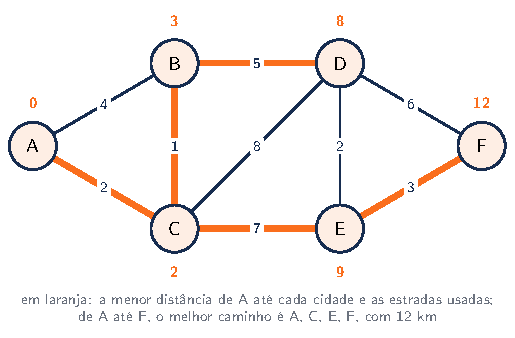
\includegraphics[width=0.8\linewidth,keepaspectratio]{imagens/capitulo-06_dijkstra.pdf}
\end{center}

A fila de prioridade do C++ é a \texttt{priority\_queue}. Por padrão ela entrega o \textbf{maior} elemento; com \texttt{greater<>}, passa a entregar o menor. Guardamos pares (distância, vértice), porque os pares são comparados primeiro pelo primeiro campo. Por dentro, ela é um \textit{heap}, estrutura que você vai construir no Capítulo 8, e insere e retira em $O(\log n)$.

\begin{codigo}
\begin{Verbatim}[breaklines=true, breaksymbolleft={}, fontsize=\footnotesize]
// trecho
vector<int> dijkstra(const Grafo &g, int origem, vector<int> &anterior) {
    vector<int> distancia(g.vertices(), INFINITO);
    anterior.assign(g.vertices(), -1);
    priority_queue<pair<int, int>, vector<pair<int, int>>, greater<>> fila;   // (distância, vértice)
    distancia[origem] = 0;
    fila.push({0, origem});
    while (!fila.empty()) {
        auto [d, v] = fila.top();               // o mais próximo ainda na fila
        fila.pop();
        if (d > distancia[v]) continue;         // registro antigo: já achamos caminho melhor
        for (const Aresta &a : g.vizinhos(v)) {
            int nova = d + a.peso;
            if (nova < distancia[a.destino]) {  // relaxa a aresta
                distancia[a.destino] = nova;
                anterior[a.destino] = v;
                fila.push({nova, a.destino});
            }
        }
    }
    return distancia;
}
\end{Verbatim}
\end{codigo}

Um vértice pode entrar na fila mais de uma vez, sempre que sua distância melhora. A linha \texttt{if (d > distancia[v]) continue;} descarta as entradas antigas, que ficaram desatualizadas. Com lista de adjacência e \textit{heap}, o custo é $O((V + E) \log V)$.

\begin{destaque}{Pesos negativos}
O Dijkstra só funciona com pesos \textbf{maiores ou iguais a zero}. Com um peso negativo, um vértice já tratado como definitivo poderia ficar mais perto depois, por um caminho que passa pela aresta negativa, e o algoritmo não volta para corrigir. Para esses grafos existe o algoritmo de Bellman-Ford, mais lento: $O(V \cdot E)$.
\end{destaque}

\subsection{6.6 Árvore geradora mínima}

Agora o problema é outro. A prefeitura quer asfaltar estradas de modo que seja possível ir de qualquer cidade a qualquer outra, gastando o mínimo possível. Não é preciso asfaltar todas: basta escolher um conjunto de estradas que \textbf{conecte todos os vértices} com a \textbf{menor soma de pesos}. Esse conjunto não terá ciclos (um ciclo sempre tem uma estrada dispensável), então será uma árvore com $V - 1$ arestas, chamada \textbf{árvore geradora mínima} (AGM, ou MST, do inglês \textit{minimum spanning tree}).

\begin{center}
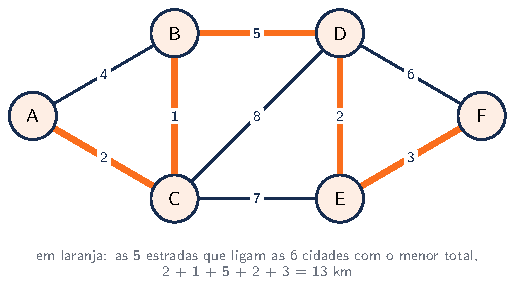
\includegraphics[width=0.8\linewidth,keepaspectratio]{imagens/capitulo-06_agm.pdf}
\end{center}

Compare com a figura do Dijkstra: as respostas são diferentes. A AGM usa a estrada D-E e não a C-E, porque o objetivo dela é o menor \textbf{total} da rede, e não o menor caminho a partir de uma cidade. Para ir de A até F pela AGM, você percorreria $2 + 1 + 5 + 2 + 3 = 13$ km, mais do que os 12 km do Dijkstra.

O \textbf{algoritmo de Prim} constrói a AGM a partir de um vértice qualquer. A cada passo, ele escolhe a aresta \textbf{mais barata} que liga a árvore já construída a um vértice ainda de fora. É, de novo, um trabalho para a fila de prioridade, agora guardando (peso, de onde, para onde):

\begin{codigo}
\begin{Verbatim}[breaklines=true, breaksymbolleft={}, fontsize=\footnotesize]
// trecho
int prim(const Grafo &g, vector<pair<int, int>> &escolhidas) {
    vector<bool> naArvore(g.vertices(), false);
    priority_queue<tuple<int, int, int>, vector<tuple<int, int, int>>, greater<>> fila;   // (peso, de, para)
    fila.push({0, -1, 0});                      // começa pelo vértice 0, sem aresta
    int total = 0;
    while (!fila.empty()) {
        auto [peso, de, v] = fila.top();        // a aresta mais barata disponível
        fila.pop();
        if (naArvore[v]) continue;              // criaria um ciclo
        naArvore[v] = true;
        total += peso;
        if (de != -1) escolhidas.push_back({de, v});
        for (const Aresta &a : g.vizinhos(v)) {
            if (!naArvore[a.destino]) fila.push({a.peso, v, a.destino});
        }
    }
    return total;
}
\end{Verbatim}
\end{codigo}

O Prim é um \textbf{algoritmo guloso}: a cada passo, faz a escolha que parece melhor naquele momento, sem voltar atrás, e mesmo assim chega à melhor resposta. Você vai estudar essa família de algoritmos no Capítulo 9, junto com o \textbf{algoritmo de Kruskal}, outra forma gulosa de construir a AGM. O custo do Prim com \textit{heap} também é $O((V + E) \log V)$.

Este é o programa completo dos dois algoritmos:

\begin{codigo}
\begin{Verbatim}[breaklines=true, breaksymbolleft={}, fontsize=\footnotesize]
#include <vector>
#include <queue>
#include <tuple>
#include <limits>       // numeric_limits
#include <functional>   // greater
#include <algorithm>    // reverse

struct Aresta {
    int destino;
    int peso;
};

class Grafo {
private:
    vector<vector<Aresta>> adjacentes;   // uma lista de vizinhos por vértice

public:
    explicit Grafo(int n) : adjacentes(n) {}

    int vertices() const { return static_cast<int>(adjacentes.size()); }

    void ligar(int a, int b, int peso = 1) {   // aresta não dirigida
        adjacentes[a].push_back({b, peso});
        adjacentes[b].push_back({a, peso});
    }

    const vector<Aresta> &vizinhos(int v) const { return adjacentes[v]; }
};

const string NOMES = "ABCDEF";
const int INFINITO = numeric_limits<int>::max();

vector<int> dijkstra(const Grafo &g, int origem, vector<int> &anterior) {
    vector<int> distancia(g.vertices(), INFINITO);
    anterior.assign(g.vertices(), -1);
    priority_queue<pair<int, int>, vector<pair<int, int>>, greater<>> fila;   // (distância, vértice)
    distancia[origem] = 0;
    fila.push({0, origem});
    while (!fila.empty()) {
        auto [d, v] = fila.top();               // o mais próximo ainda na fila
        fila.pop();
        if (d > distancia[v]) continue;         // registro antigo: já achamos caminho melhor
        for (const Aresta &a : g.vizinhos(v)) {
            int nova = d + a.peso;
            if (nova < distancia[a.destino]) {  // relaxa a aresta
                distancia[a.destino] = nova;
                anterior[a.destino] = v;
                fila.push({nova, a.destino});
            }
        }
    }
    return distancia;
}

string caminho(const vector<int> &anterior, int destino) {
    string resultado;
    for (int v = destino; v != -1; v = anterior[v]) {   // volta pelos anteriores
        resultado += NOMES[v];
    }
    reverse(resultado.begin(), resultado.end());        // da origem ao destino
    return resultado;
}

int prim(const Grafo &g, vector<pair<int, int>> &escolhidas) {
    vector<bool> naArvore(g.vertices(), false);
    priority_queue<tuple<int, int, int>, vector<tuple<int, int, int>>, greater<>> fila;   // (peso, de, para)
    fila.push({0, -1, 0});                      // começa pelo vértice 0, sem aresta
    int total = 0;
    while (!fila.empty()) {
        auto [peso, de, v] = fila.top();        // a aresta mais barata disponível
        fila.pop();
        if (naArvore[v]) continue;              // criaria um ciclo
        naArvore[v] = true;
        total += peso;
        if (de != -1) escolhidas.push_back({de, v});
        for (const Aresta &a : g.vizinhos(v)) {
            if (!naArvore[a.destino]) fila.push({a.peso, v, a.destino});
        }
    }
    return total;
}

int main() {
    enum { A, B, C, D, E, F };
    Grafo mapa(6);
    mapa.ligar(A, B, 4);
    mapa.ligar(A, C, 2);
    mapa.ligar(B, C, 1);
    mapa.ligar(B, D, 5);
    mapa.ligar(C, D, 8);
    mapa.ligar(C, E, 7);
    mapa.ligar(D, E, 2);
    mapa.ligar(D, F, 6);
    mapa.ligar(E, F, 3);

    vector<int> anterior;
    vector<int> distancia = dijkstra(mapa, A, anterior);
    for (int v = 0; v < mapa.vertices(); v++) {
        cout << NOMES[v] << ": " << distancia[v] << " km, " << caminho(anterior, v) << endl;
    }
    // A: 0 km, A     B: 3 km, ACB    C: 2 km, AC
    // D: 8 km, ACBD  E: 9 km, ACE    F: 12 km, ACEF

    vector<pair<int, int>> escolhidas;
    int total = prim(mapa, escolhidas);
    for (const auto &[de, para] : escolhidas) {
        cout << NOMES[de] << "-" << NOMES[para] << " ";
    }
    cout << endl;                                   // A-C C-B B-D D-E E-F
    cout << "Total: " << total << " km" << endl;    // Total: 13 km
}
\end{Verbatim}
\end{codigo}

Os dois algoritmos são quase iguais: a diferença está no que vai para a fila. O Dijkstra prioriza a distância \textbf{acumulada desde a origem} (\texttt{d + a.peso}); o Prim prioriza apenas o \textbf{peso da aresta} (\texttt{a.peso}).

\begin{center}
\begin{tabular}{@{}p{0.3\linewidth}p{0.36\linewidth}p{0.22\linewidth}@{}}
\toprule
\rowcolor{headergray}
\tblheader{Algoritmo} & \tblheader{Resolve} & \tblheader{Custo} \\
\midrule
BFS & menor número de arestas; percorrer & $O(V + E)$ \\
\rowcolor{rowgray} DFS & percorrer; componentes; ciclos & $O(V + E)$ \\
Kahn & ordenação topológica & $O(V + E)$ \\
\rowcolor{rowgray} Dijkstra & menor caminho com pesos $\ge 0$ & $O((V + E) \log V)$ \\
Prim & árvore geradora mínima & $O((V + E) \log V)$ \\
\bottomrule
\end{tabular}
\end{center}

\begin{destaque}{Comparando com Python}
Em Python, um grafo costuma ser um dicionário que leva cada vértice à lista de seus vizinhos, e os vértices podem ser os próprios nomes, sem precisar de índices. A fila da BFS é o \texttt{deque} do Capítulo 4, e a fila de prioridade do Dijkstra é o módulo \texttt{heapq}, que mantém uma lista comum organizada como \textit{heap} (sempre com o menor na frente):

\begin{codigo}
\begin{Verbatim}[breaklines=true, breaksymbolleft={}, fontsize=\footnotesize]
import heapq
from collections import deque

mapa = {
    'A': [('B', 4), ('C', 2)],
    'B': [('A', 4), ('C', 1), ('D', 5)],
    'C': [('A', 2), ('B', 1), ('D', 8), ('E', 7)],
    'D': [('B', 5), ('C', 8), ('E', 2), ('F', 6)],
    'E': [('C', 7), ('D', 2), ('F', 3)],
    'F': [('D', 6), ('E', 3)],
}

def largura(grafo, origem):
    distancia = {origem: 0}
    fila = deque([origem])
    while fila:
        v = fila.popleft()
        for vizinho, _ in grafo[v]:
            if vizinho not in distancia:
                distancia[vizinho] = distancia[v] + 1
                fila.append(vizinho)
    return distancia

def dijkstra(grafo, origem):
    distancia = {v: float('inf') for v in grafo}
    distancia[origem] = 0
    fila = [(0, origem)]
    while fila:
        d, v = heapq.heappop(fila)
        if d > distancia[v]:
            continue
        for vizinho, peso in grafo[v]:
            if d + peso < distancia[vizinho]:
                distancia[vizinho] = d + peso
                heapq.heappush(fila, (d + peso, vizinho))
    return distancia

print(largura(mapa, 'A'))    # {'A': 0, 'B': 1, 'C': 1, 'D': 2, 'E': 2, 'F': 3}
print(dijkstra(mapa, 'A'))   # {'A': 0, 'B': 3, 'C': 2, 'D': 8, 'E': 9, 'F': 12}
\end{Verbatim}
\end{codigo}

O \texttt{float('inf')} faz o papel do ``infinito'' e, como em Python os inteiros não têm limite, não existe o risco de estouro que existe no C++ ao somar um peso a \texttt{numeric\_limits<int>::max()}. Para grafos grandes, a biblioteca externa \texttt{networkx} já traz todos esses algoritmos prontos.
\end{destaque}

\subsection{Erros Comuns}

\begin{itemize}
  \item \textbf{Esquecer de marcar os visitados.} Em um grafo com ciclos, a busca volta a vértices já vistos e entra em um laço sem fim, ou em uma recursão que estoura a pilha.
  \item \textbf{Marcar na hora errada na BFS.} Marque o vértice quando ele \textit{entra} na fila, e não quando sai. Do contrário, o mesmo vértice pode ser colocado na fila várias vezes.
  \item \textbf{Ligar a aresta em um só sentido em um grafo não dirigido.} Cada aresta precisa aparecer na lista dos dois vértices. Esquecer uma das duas transforma o grafo em dirigido sem você perceber.
  \item \textbf{Usar matriz de adjacência em grafos grandes e esparsos.} A memória cresce com $V^2$; com cem mil vértices, já são dez bilhões de posições.
  \item \textbf{Usar a BFS para o caminho mínimo em grafo ponderado.} A BFS conta arestas, não soma pesos. Com pesos, use o Dijkstra.
  \item \textbf{Usar o Dijkstra com pesos negativos.} O resultado pode sair errado, sem nenhum aviso.
  \item \textbf{Somar ao ``infinito''.} Em C++, \texttt{numeric\_limits<int>::max() + 1} estoura. Só some a distâncias que já não sejam infinitas, como o Dijkstra faz ao partir apenas de vértices retirados da fila.
  \item \textbf{Esquecer o \texttt{greater<>} na \texttt{priority\_queue}.} Sem ele, a fila entrega o \textit{maior} elemento primeiro, e o Dijkstra e o Prim dão respostas erradas.
  \item \textbf{Confundir caminho mínimo com árvore geradora mínima.} São problemas diferentes, com respostas diferentes, como as duas figuras do capítulo mostram.
\end{itemize}
